\title{Python Sheet}
\date{\today}
\author{Benjamin Bucheli}
\documentclass[10pt,twoside,a4paper,fleqn,xcolor=table]{scrartcl}

%%%%%%%%%%%%%%%%%%%%%%%%%%%%%%%%%%%%%%%%%%%%%
% Standard Header für 
% - Makros 
% - Farben
% - Mathematische Operatoren
%%%%%%%%%%%%%%%%%%%%%%%%%%%%%%%%%%%%%%%
%% Makros & anderer Low-Level bastel %%
%%%%%%%%%%%%%%%%%%%%%%%%%%%%%%%%%%%%%%%
\makeatletter
%% Makros für Titel, Autor und Datum 
%% Dank diesem Makro stehen Titel, Autor und Datum überall im Dokument zur verfügung
%% Date hat zudem den Default-Wert \today
\def\@Title{}
\def\@Author{}
\def\@Date{\today}
\newcommand{\Title}{\@Title}
\newcommand{\Author}{\@Author}
\newcommand{\Date}{\@Date}
\AtBeginDocument{%
  \let\@Title\@title
  \let\@Author\@author
  \let\@Date\@date
}

%% Makros für den Arraystretch (bei uns meist in Tabellen genutzt, welche Formeln enthalten)
% Default Value
\def\@ArrayStretchDefault{1} % Entspricht der Voreinstellung von Latex

% Setzt einen neuen Wert für den arraystretch
\newcommand{\setArrayStretch}[1]{\renewcommand{\arraystretch}{#1}}

% Setzt den arraystretch zurück auf den default wert
\newcommand{\resetArrayStretch}{\renewcommand{\arraystretch}{\@ArrayStretchDefault}}

% Makro zum setzten des Default arraystretch. Kann nur in der Präambel verwendet werden.
\newcommand{\setDefaultArrayStretch}[1]{%
	\AtBeginDocument{%
		\def\@ArrayStretchDefault{#1}
		\renewcommand{\arraystretch}{#1}
	}
}
\makeatother


%%%%%%%%%%%%%%%%%%%%%%%
%% Wichtige Packages %%
%%%%%%%%%%%%%%%%%%%%%%%
\usepackage[utf8]{inputenc} % UTF-8 unterstützung
\usepackage[english, ngerman]{babel} % Silbentrennung
%\usepackage[automark]{scrpage2} % Header und Footer
%\RequirePackage{scrlfile}
%\ReplacePackage{scrpage2}{scrlayer-scrpage}
\usepackage{tabularx}

% Für Abbildungen mit mehreren kleinen Bilder
% Doku: http://www.ctan.org/tex-archive/macros/latex/contrib/caption/
\usepackage[justification=centering]{caption}
\usepackage{subcaption}

\ifx\GUARDlistings\undefined
\def\GUARDlistings{}

\usepackage{color}

\definecolor{mygreen}{rgb}{0,0.6,0}
\definecolor{mygray}{rgb}{0.5,0.5,0.5}
\definecolor{mymauve}{rgb}{0.58,0,0.82}
\definecolor{bgGray}{rgb}{0.9,0.9,0.9}
\definecolor{darkGray}{rgb}{0.25,0.25,0.25}
\definecolor{myorange}{rgb}{1, 0.3, 0}
\definecolor{numberBlue}{rgb}{0.4, 0.7, 1}
\definecolor{numberYellow}{rgb}{1,0.9,0.1}

\usepackage{listings}
\lstset{ %
    firstnumber=1,
    backgroundcolor=\color{gray!10},   % choose the background color; you must add        \usepackage{color} or \usepackage{xcolor}
    basicstyle=\normalsize\ttfamily, % the size of the fonts that are used for the code
    breakatwhitespace=false,         % sets if automatic breaks should only happen at whitespace
    breaklines=true,                 % sets automatic line breaking
    captionpos=b,                    % sets the caption-position to bottom
    commentstyle=\color{mygreen},    % comment style
    deletekeywords={...},            % if you want to delete keywords from the given language
    otherkeywords={},             % if you want to add more keywords to the set
    escapeinside={\%*}{*\%},          % if you want to add LaTeX within your code
    extendedchars=true,              % lets you use non-ASCII characters; for 8-bits encodings only, does not work with UTF-8
    frame=tb,	                 % adds a frame around the code
    keepspaces=true,                 % keeps spaces in text, useful for keeping indentation of code (possibly needs columns=flexible)
    keywordstyle=\color{blue},       % keyword style
    language=C++,                    % the language of the code   
    numbers=none,                    % where to put the line-numbers; possible values are (none, left, right)
    numbersep=5pt,                   % how far the line-numbers are from the code
    numberstyle=\tiny\color{mygray}, % the style that is used for the line-numbers
    rulecolor=\color{black},         % if not set, the frame-color may be changed on line-breaks within not-black text (e.g. comments (green here))
    showspaces=false,                % show spaces everywhere adding particular underscores; it overrides 'showstringspaces'
    showstringspaces=false,          % underline spaces within strings only
    showtabs=false,                  % show tabs within strings adding particular underscores
    stepnumber=2,                    % the step between two line-numbers. If it's 1, each line will be numbered
    stringstyle=\color{mymauve},     % string literal style
    tabsize=4,	                     % sets default tabsize to 2 spaces
    %title=\lstname                   % show the filename of files included with         \lstinputlisting; also try caption instead of title
}

\lstdefinestyle{Java}{
	belowcaptionskip=1\baselineskip,
	breaklines=true,
	language=Java,
	showstringspaces=false,
	otherkeywords={@Override, var},
	keywordstyle=\color{myorange},
	commentstyle=\color{mymauve},
	identifierstyle=\color{black},
	stringstyle=\color{mygreen},
	numberstyle=\color{numberBlue},
	tabsize=4
}

\lstdefinestyle{C}{
  numbers=left,
  belowcaptionskip=1\baselineskip,
  breaklines=true,
  frame=L,
  xleftmargin=10pt,
  language=C,
  showstringspaces=false,
  basicstyle=\footnotesize\ttfamily,
  keywordstyle=\bfseries\color{green!40!black},
  commentstyle=\itshape\color{purple!40!black},
  identifierstyle=\color{blue},
  stringstyle=\color{orange},
  numberstyle=\ttfamily\tiny,
  tabsize=2
}

\lstdefinestyle{Cpp}{
  numbers=left,
  belowcaptionskip=1\baselineskip,
  breaklines=true,
  frame=L,
  xleftmargin=10pt,
  language=C++,
  showstringspaces=false,
  basicstyle=\footnotesize\ttfamily,
  keywordstyle=\bfseries\color{green!40!black},
  commentstyle=\itshape\color{purple!40!black},
  identifierstyle=\color{blue},
  stringstyle=\color{orange},
  numberstyle=\ttfamily\tiny,
  tabsize=2
}

\lstdefinestyle{Python}{
	belowcaptionskip=1\baselineskip,
	breaklines=true,
	language=Python,
	showstringspaces=false,
	keywordstyle=\color{mymauve},
	emph={print,input,all,next},
	emphstyle={\color{myorange}},
	commentstyle=\color{darkGray},
	identifierstyle=\color{black},
	stringstyle=\color{mygreen},
	morestring=[b]{"""},
	numberstyle=\color{numberYellow},
	tabsize=4
}


% Seitenränder
\usepackage[left=1cm,right=1cm,top=0.5cm,bottom=0.5cm,includeheadfoot]{geometry}

\usepackage[table]{xcolor}
\usepackage{hyperref}
\usepackage{longtable}
\usepackage{multirow} % Create tabular cells spanning multiple rows
\usepackage{multicol} % In­ter­mix sin­gle and mul­ti­ple columns
\usepackage{rotating} % Rotation tools, including rotated fullpage floats
\usepackage{enumitem}
\usepackage{graphicx}
\usepackage{graphbox} % Align Images
\usepackage{bold-extra} % for usage of both \textbf and \texttt on one word
\usepackage[export]{adjustbox}	% Align Images 

%%%%%%%%%%%%%%%%%%%%%%%%%%%%%%%%%%%
%% Layout der Kopf und Fusszeile %%
%%%%%%%%%%%%%%%%%%%%%%%%%%%%%%%%%%%
\usepackage[headsepline,footsepline]{scrlayer-scrpage}
\pagestyle{scrheadings}

\ohead{\pagemark}
\chead{FS21}
\ihead{Python Sheet}

\ofoot{\today}
\ifoot{F.Baumgartner, B.Bucheli}

%%%%%%%%%%%%%%%%%%%%%%%%%%%%%%%%%%%%%%%%%%%%%

\begin{document}
	\lstset{style=Python}
	\vspace{-0.5cm}
\section*{Generell}
Die numerischen Datentypen sind gleichermaßen zu behandeln wie in den bekannten Programmiersprachen.

	\begin{minipage}[t]{12.5cm}
		\subsection*{Datentypen}
			\rowcolors{1}{blue!10}{white}
			\begin{tabular}{|>{\bfseries}l l l|}
				\hline Datentyp & \bfseries{Beschreibung} & \bfseries{False-Wert}
				\\\hline NoneType & Indikator für nichts & None
				\\\hline \multicolumn{3}{|l|}{\bfseries{Numerische Datentypen}}
				\\ int & Ganze Zahlen & 0
				\\ float & Gleitkommazahlen & 0.0
				\\ bool & Boolesche Werte & False
				\\ complex & Komplexe Zahlen & 0 + 0j
				\\\hline \multicolumn{3}{|l|}{\bfseries{Sequenzielle Datentypen}}
				\\ str & Zeichenketten oder Strings(unveränderlich) & ' '
				\\ list & Listen(veränderlich) & []
				\\ tuple & Tupel(unveränderlich) & ()
				\\ bytes & Sequenz von Bytes(unveränderlich) & b' '
				\\ bytesarray & Sequenz von Bytes(veränderlich) & bytearray(b' ')
				\\\hline Mengen & & 
				\\ set & Einmalig vorkommende Objekte & set()
				\\ frozenset & Wie set jedoch unveränderlich & frozenset()
				\\\hline \multicolumn{3}{|l|}{\bfseries{Assoziative Datentypen}}
				\\ dict & Dictionary(veränderlich) & { }
				\\\hline
			\end{tabular}
	\end{minipage}
		%\hspace*{1cm}
		\begin{minipage}[t]{3cm}
			%\vspace*{0.7cm}
			\subsection*{Operatoren}
				\rowcolors{1}{blue!10}{white}
				\begin{tabular}{|l l|}
					\hline \bfseries{Operator} & \bfseries{Beschreibung} \\\hline
					x // y & Ganzzahliger Quotient\\
					x ** y & Potenzieren, $x^y$ \\ 
					+,-,... & Übliche Operation\\\hline
				\end{tabular}
			\subsection*{Variablen}
				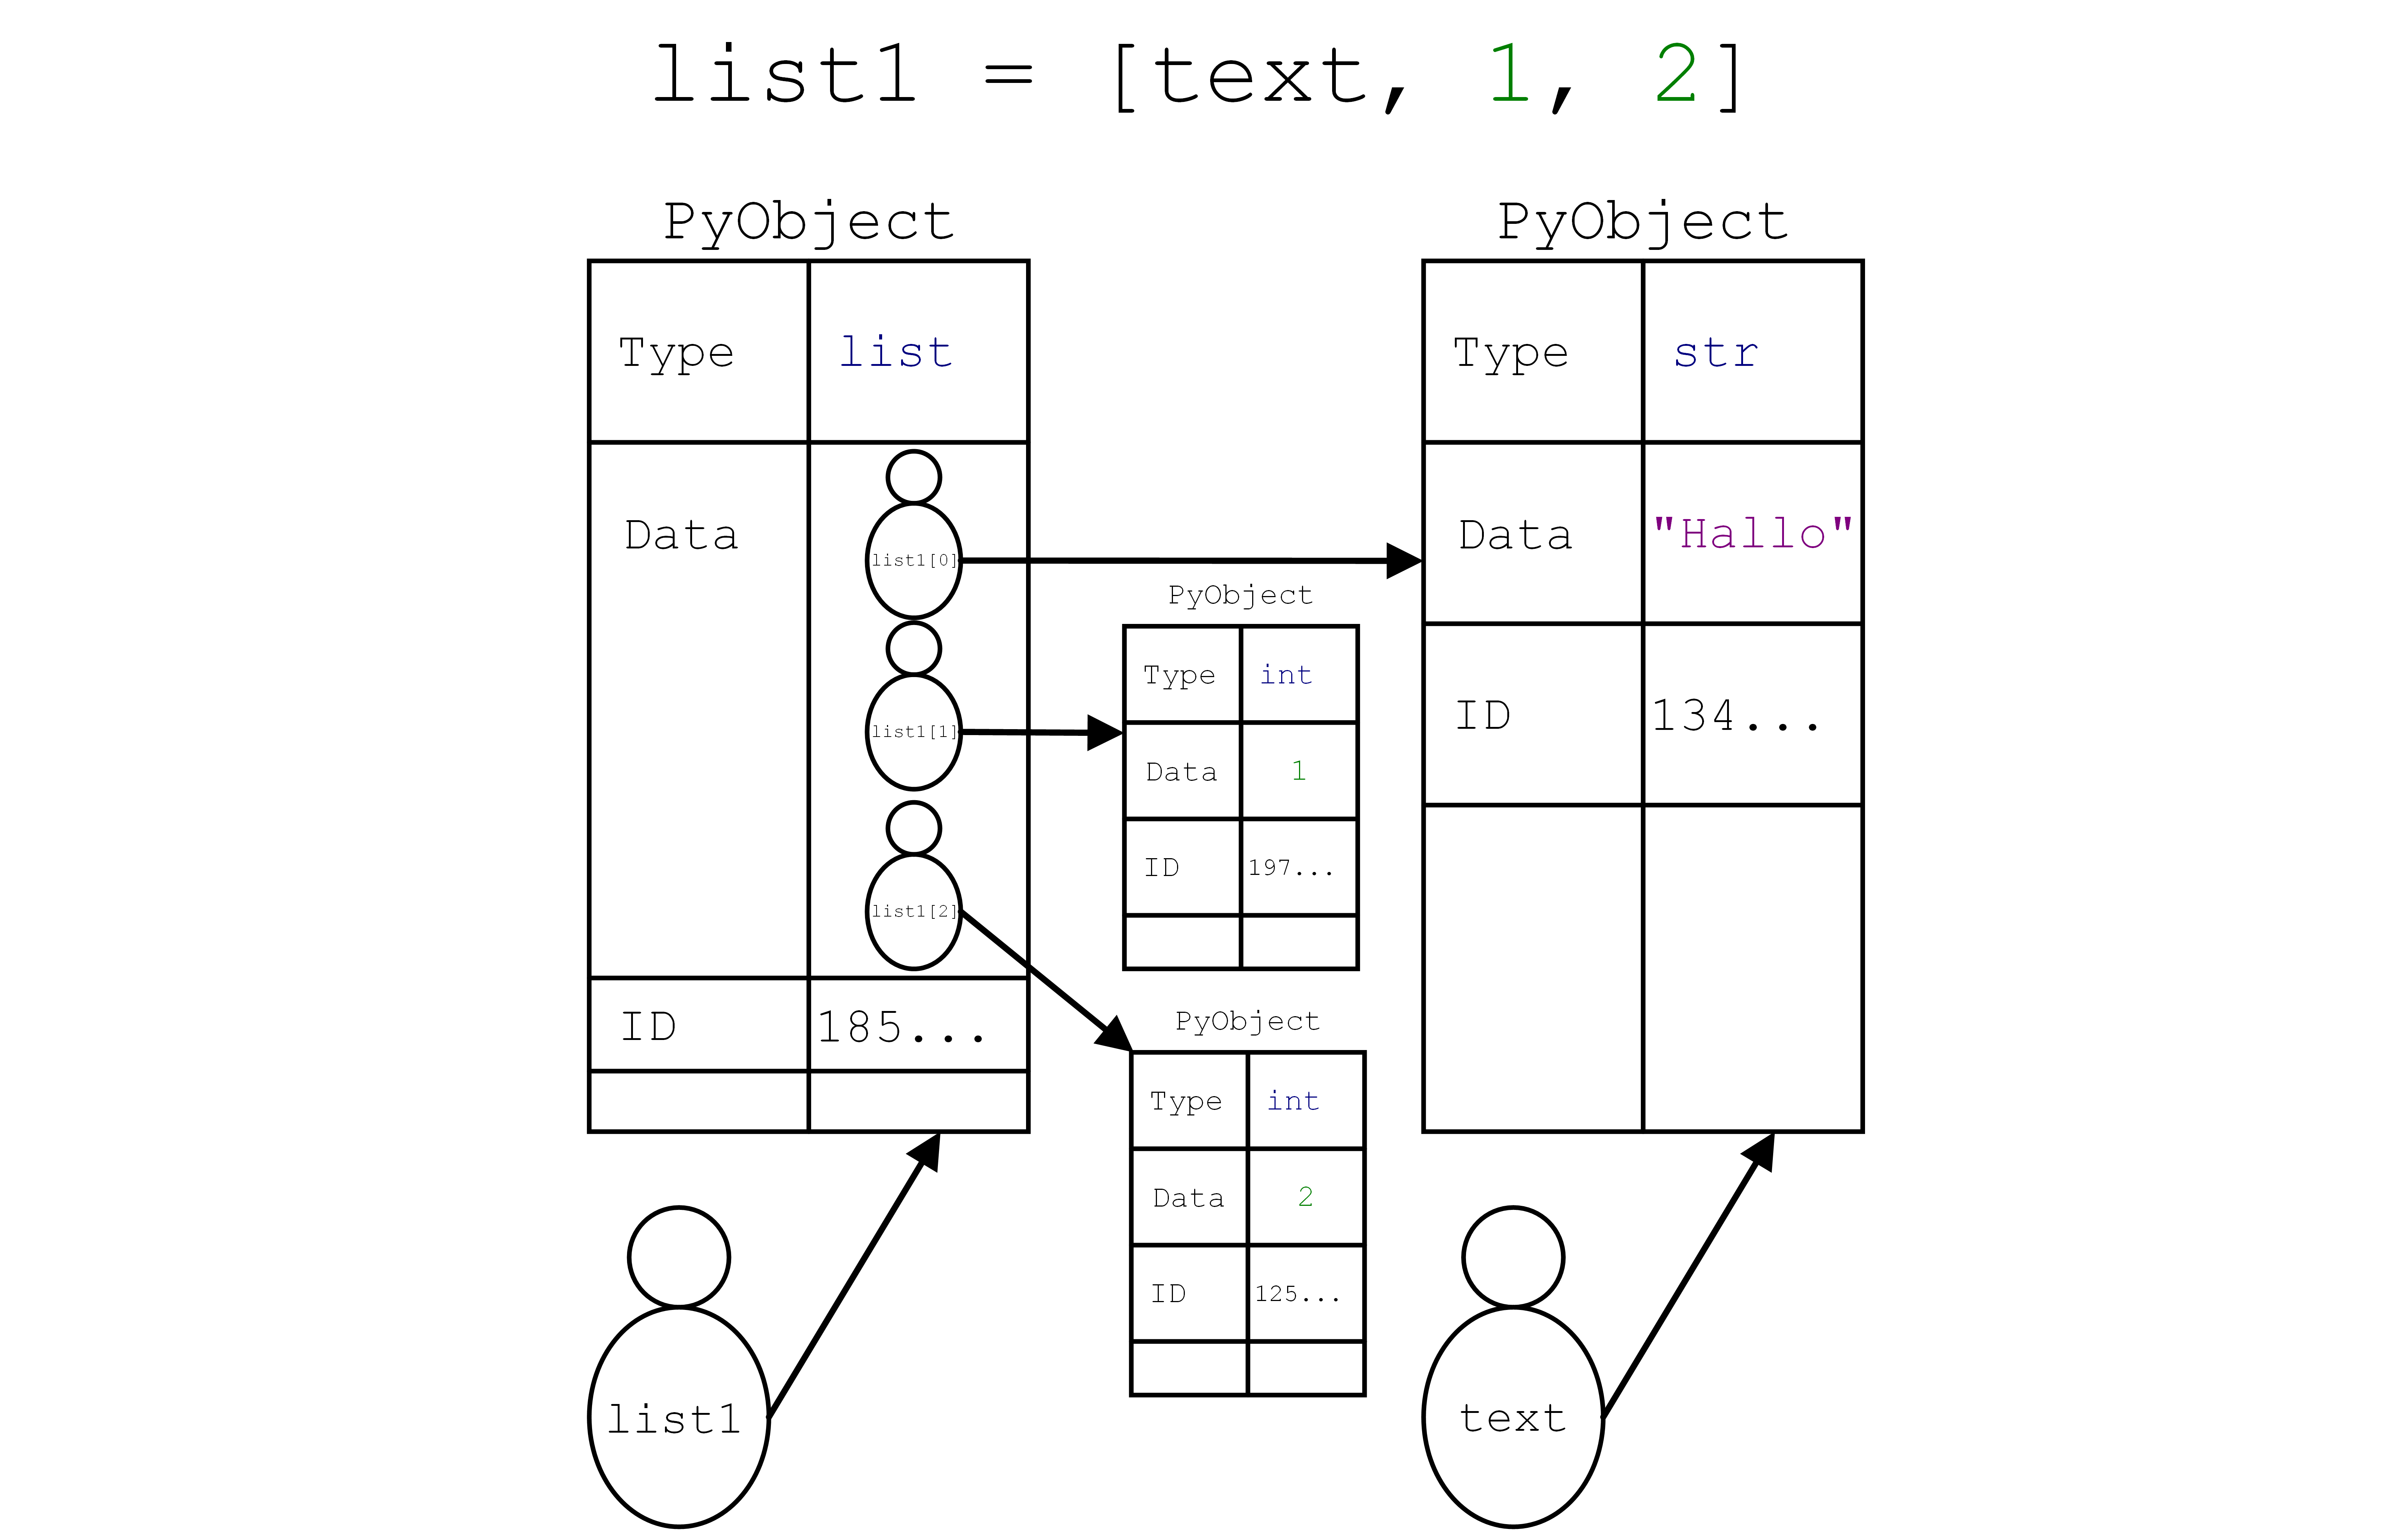
\includegraphics[height=4.5cm, align=t]{pics/Variablen.PNG}
		\end{minipage}
	\subsection*{Casting}
	\hspace{2cm}
	\rowcolors{1}{blue!10}{white}
	\begin{tabular}{|l l l | l l l|}
		\hline \bfseries{Datentyp} & \bfseries{Klasse} & \bfseries{Direkt} & \bfseries{Datentyp} & \bfseries{Klasse} & \bfseries{Direkt}
		\\\hline Ganzzahl & int() & 3 & Gleitkommazahl & float() & 3.1415
		\\ Boolescher Wert & bool() & True,False & Komplexe Zahl & complex() & 2 + 4j
		\\ String & str() & "HSR",'OST' & Liste & list() & [1,2,3]
		\\  Menge & set() & {1,2,3} & Tupel & tuple() & (1,2,3)
		\\ Unver. Menge & frozenset() & frozenset({1,2,3}) & Dictionary & dict() & {}, {"Key": 1}
		\\\hline
	\end{tabular}
	\subsection*{Eingabe und Ausgabe}
		\begin{minipage}[h]{7cm}
			\lstinputlisting{code/Streams.py}
		\end{minipage}
		\begin{minipage}[h]{8cm}
		\rowcolors{1}{blue!10}{white}
			\begin{tabular}{|l l l|}
				\hline \bfseries{Parameter} & \bfseries{Beschreibung} & \bfseries{Default}
				\\\hline object(s) & Alle Objekte werden in String konvertiert & 
				\\ sep='seperator' & Separierung der Objekte & ' '
				\\ end='end' & Letztes Zeichen des print-Befehl & '\textbackslash n'
				\\ file & Objekt mit einer Write-Methode & sys.stdout
				\\ flush & Boolscher Wert für die Output-Überprüfung & False
				\\\hline
			\end{tabular}
		\end{minipage}
	\section*{Listen}
\lstinputlisting{code/Listen.py}

	\section*{Tupel}
\lstinputlisting{code/Tupel.py}
	\section*{Set}
%%%%%%%%%%%%%%%%%%%%%%%%%%%%%%%%%%%%%%%%%%%%%%%%%%
\hspace{1cm}
\rowcolors{1}{blue!10}{white}
\begin{tabular}{|l l l|}
	\hline set.add(elem) & set.intersection(*others) $\to$ set & set.remove(elem)
	\\ set.clear() & set.intersection\_update(*others) & set.symmetric\_difference(other) $\to$ set
	\\ set.copy() $\to$ set & set.isdisjoint(other) $\to$ bool & set.symmetric\_difference\_update(other)
	\\ set.difference(*others) $\to$ set & set.issubset(other) $\to$ bool & set.union(*others) $\to$ set
	\\ set.difference\_update(*others) & set.issuperset(other) $\to$ bool & set.update(*others)
	\\ set.discard(elem) & set.pop() $\to$ object &
	\\\hline
\end{tabular}
%%%%%%%%%%%%%%%%%%%%%%%%%%%%%%%%%%%%%%%%%%%%%%%%%%
\vspace{0.1cm}
\\
Ein set kann ebenfalls wie eine Liste behandelt werden, wobei die Werte nur einmalig vorkommen können und sie nicht veränderbar sind. Weitere Werte können hinzugefügt oder entfernt werden.
Sets sind ungeordnet, heisst, \\\textcolor{red}{die Reihenfolge der Elemente kann nicht vorhergesagt werden.}
\vspace{0.5cm}
\\
\vspace{0.1cm}
\textbf{Erzeugen}\\
\begin{minipage}[h]{10cm}
	\lstinputlisting{code/Set/Set_create.py}
\end{minipage}
\begin{minipage}[h]{8cm}
	\textcolor{red}{\textbf{Out:}}
	\\myset = {'I', 'cheese', 'love', 'swiss'}
	\\aset = {'six', 'two', 'one'}
\end{minipage}
%%%%%%%%%%%%%%%%%%%%%%%%%%%%%%%%%%%%%%%%%%%%%%%%%%
\\
\vspace{0.1cm}
\textbf{Basics}\\
\begin{minipage}[h]{10cm}
	\lstinputlisting{code/Set/Set_basic.py}
\end{minipage}
\begin{minipage}[h]{8cm}
	\textcolor{red}{\textbf{Out:}}
	\\myset = {12, 77, 'elem'}
	\\myset = set()
	\\aset = {'elem', 12, 77}
\end{minipage}
%%%%%%%%%%%%%%%%%%%%%%%%%%%%%%%%%%%%%%%%%%%%%%%%%%
	\section*{Dictionary}
	\begin{minipage}[h]{9cm}
		\lstinputlisting{Code/Dictionary.py}
	\end{minipage}
	\begin{minipage}[h]{10cm}
		\rowcolors{1}{blue!10}{white}
		\begin{tabular}{|l l|}
			\hline \bfseries{Methode} & \bfseries{Beschreibung}
			\\\hline clear() & Alle Elemente entfernen
			\\ copy() & Kopiert das Dictionary
			\\ keys() & Gibt eine Liste mit den Schlüsselwerten
			\\ items() & Gibt eine Liste mit tuple für alle keys
			\\ values() & Gibt eine Liste mit allen Werte zurück
			\\\hline
		\end{tabular}
	\end{minipage}
	\section*{Strings}
	\begin{minipage}[h]{7cm}
		\lstinputlisting{Code/Strings.py}
	\end{minipage}
	\begin{minipage}[h]{7cm}
		\lstinputlisting{Code/Fstrings.py}
	\end{minipage}
\newpage

	\newpage
\section*{Matplotlib}
\rowcolors{1}{blue!10}{white}
\begin{tabular}{|l|}
	\hline \bfseries{Creation}
	\\\parbox{18cm}{plt.figure(num=None, dpi=None, facecolor=None, edgecolor=Nonem frameon=True, FigureClass=<class "matplotlib.figure.Figure">, clear=False, **kwargs) $\to$ Figure)}
	\\plt.subplot(*args, **kwargs) $\to$ AxesSubplot
	\\\parbox{18cm}{plt.subplots(nrows=1, ncols=1, *, sharex=False, sharey=False, squeeze=True, subplot kw=None, gridspec kw=None, **fig kw) Figure, $\to$  axes.Axes}
	\\plt.twinx(ax=None) $\to$ AxesSubplot
	\\plt.twiny(ax=None) $\to$ AxesSubplot
	\\plt.tight layout(*, pad=1.08, h pad=None, w pad=None, rect=None)
	\\plt.savefig(*args, **kwargs)
	\\plt.show(*, block=None)
	\\\hline\bfseries{Drawing}
	\\plt.annotate(text, xy, *args, **kwargs) $\to$ Annotation
	\\plt.arrow(x, y, dx, dy, **kwargs) $\to$ FancyArrow
	\\plt.contour(*args, data=None, **kwargs) $\to$ QuadContourSet
	\\plt.contourf(*args, data=None, **kwargs) $\to$ QuadContourSet
	\\plt.loglog(*args, **kwargs) $\to$ list of Line2D objects
	\\\parbox{18cm}{plt.plot(*args, scalex=True, scaley=True, data=None, **kwargs) $\to$ list of Line2D objects}
	\\\parbox{18cm}{plt.scatter(x, y, s=None, c=None, marker=None, cmap=None, norm=None, vmin=None, vmax=None, alpha=None,
		linewidths=None, verts=<deprecated parameter>, edgecolors=None, *, plotnonfinite=False, data=None,
		**kwargs) $\to$ PathCollection}
	\\plt.semilogx(*args, **kwargs) $\to$ list of Line2D objects
	\\plt.semilogy(*args, **kwargs) $\to$ list of Line2D objects
	\\\parbox{18cm}{plt.stem(*args, linefmt=None, markerfmt=None, basefmt=None, bottom=0, label=None,
		use line collection=True, data=None) $\to$ StemContainer}
	\\\parbox{18cm}{plt.step(x, y, *args, where="pre", data=None, **kwargs) $\to$ list of Line2D objects}
	\\\parbox{18cm}{plt.streamplot(x, y, u, v, density=1, linewidth=None, color=None, cmap=None, norm=None, arrowsize=1,
		arrowstyle="-|>", minlength=0.1, transform=None, zorder=None, start points=None, maxlength=4.0,
		integration direction="both", *, data=None) $\to$ StreamplotSet}
	\\plt.text(x, y, s, fontdict=None, **kwargs) $\to$ Text
	\\\hline\bfseries{Decoration}
	\\plt.axis(*args, emit=True, **kwargs) $\to$ Annotation
	\\plt.axhline(y=0, xmin=0, xmax=1, **kwargs) $\to$ Line2D
	\\plt.axvline(x=0, ymin=0, ymax=1, **kwargs) $\to$ Line2D
	\\plt.colorbar(mappable=None, cax=None, ax=None, **kw) $\to$ Colorbar
	\\plt.grid(b=None, which="major", axis="both", **kwargs)
	\\plt.legend(*args, **kwargs)
	\\plt.margins(*margins, x=None, y=None, tight=True) $\to$ tuple
	\\plt.suptitle(t, **kwargs) Text
	\\plt.title(label, fontdict=None, loc=None, pad=None, *, y=None, **kwargs) $\to$ Text
	\\plt.xlabel(xlabel, fontdict=None, labelpad=None, *, loc=None, **kwargs)
	\\plt.xlim(*args, **kwargs) $\to$ tuple
	\\plt.xticks(ticks=None, labels=None, **kwargs) $\to$ tuple
	\\plt.ylabel(ylabel, fontdict=None, labelpad=None, *, loc=None, **kwargs)
	\\plt.ylim(*args, **kwargs) $\to$ tuple
	\\plt.yticks(ticks=None, labels=None, **kwargs) $\to$ tuple
	\\\hline\bfseries{Decoration OOP}
	\\\parbox{18cm}{Axes.set title(self, label, fontdict=None, loc=None, pad=None, *, y=None, **kwargs) $\to$ Text}
	\\\parbox{18cm}{Axes.set xlabel(self, xlabel, fontdict=None, labelpad=None, *, loc=None, **kwargs)}
	\\\parbox{18cm}{Axes.set xlim(self, left=None, right=None, emit=True, auto=False, *, xmin=None, xmax=None) $\to$ tuple}
	\\Axes.set xticks(self, ticks, *, minor=False) $\to$ tuple
	\\\parbox{18cm}{Axes.set ylabel(self, ylabel, fontdict=None, labelpad=None, *, loc=None, **kwargs)}
	\\\parbox{18cm}{Axes.set ylim(self, bottom=None, top=None, emit=True, auto=False, *, ymin=None, ymax=None) $\to$ tuple}
	\\Axes.set yticks(self, ticks, *, minor=False) $\to$ tuple
	\\\hline
\end{tabular}
\\[0.5cm]
\rowcolors{1}{blue!10}{white}
\begin{tabular}{|l l l l l l l|}
	\hline \bfseries{Linestyle} & \bfseries{Marker} & & & \bfseries{Color} & & 
	\\\hline '-', 'solid'& '.'$=$point & 'o'$=$circle & 'v'$=$triangle\_down & 'b','blue' & 'g','green' & 'r','red'
	\\':', 'dotted' & 's'$=$square & 'p'$=$pentagon & '>'$=$triangle\_right &  'c','cyan' & 'm','magenta' & 'k','black'
	\\'--', 'dashed' & '*'$=$star & 'd','D'$=$diamond & '\^'$=$triangle\_up &  'w','white' & 'y','yellow' & '\#0F0F0F'
	\\'-.', 'dashdot' & 'x','X'$=$× & '+','P'$=$plus & '<'$=$triangle\_left & (0.0, 0.5, 1.0) & & 
	\\\hline
\end{tabular}
\newpage
%%%%%%%%%%%%%%%%%%%%%%%%%%%%%%%%%%%%%%%%%%%%%%%%%%
\textbf{Einfaches Beispiel}
\\
\begin{minipage}[h]{10cm}
	\lstinputlisting{code/Matplotlib/SimpleExample.py}
\end{minipage}
\begin{minipage}[h]{8cm}
	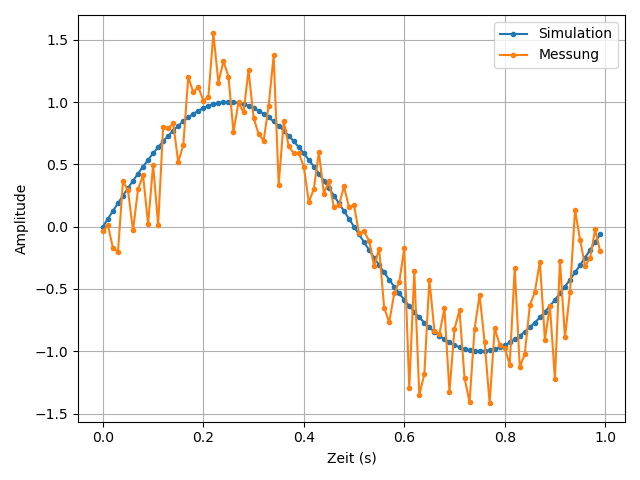
\includegraphics[width=8cm,align=t]{pics/Matplotlib/SimpleExample.png}
\end{minipage}
%%%%%%%%%%%%%%%%%%%%%%%%%%%%%%%%%%%%%%%%%%%%%%%%%%
\\[0.3cm]
%%%%%%%%%%%%%%%%%%%%%%%%%%%%%%%%%%%%%%%%%%%%%%%%%%
\textbf{OOP Beispiel}
\\
\begin{minipage}[h]{10cm}
	\lstinputlisting{code/Matplotlib/OOP_Beispiel.py}
\end{minipage}
\begin{minipage}[h]{8cm}
	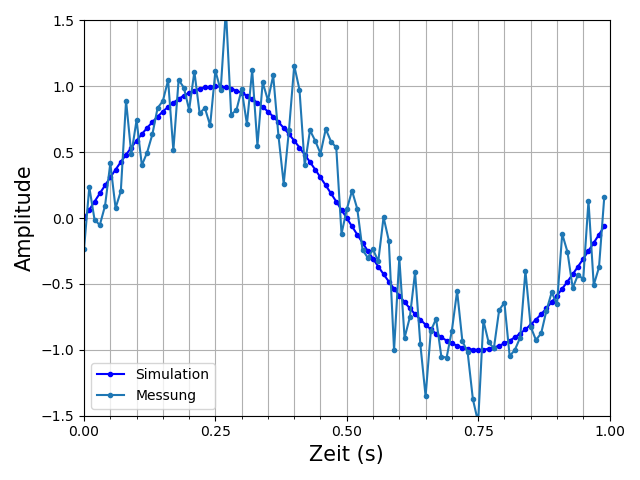
\includegraphics[width=8cm,align=t]{pics/Matplotlib/OOP_Beispiel.png}
\end{minipage}
%%%%%%%%%%%%%%%%%%%%%%%%%%%%%%%%%%%%%%%%%%%%%%%%%%
\newpage
%%%%%%%%%%%%%%%%%%%%%%%%%%%%%%%%%%%%%%%%%%%%%%%%%%
\textbf{Subplots}
\\
\begin{minipage}[h]{10cm}
	\lstinputlisting{code/Matplotlib/Subplots.py}
\end{minipage}
\begin{minipage}[h]{8cm}
	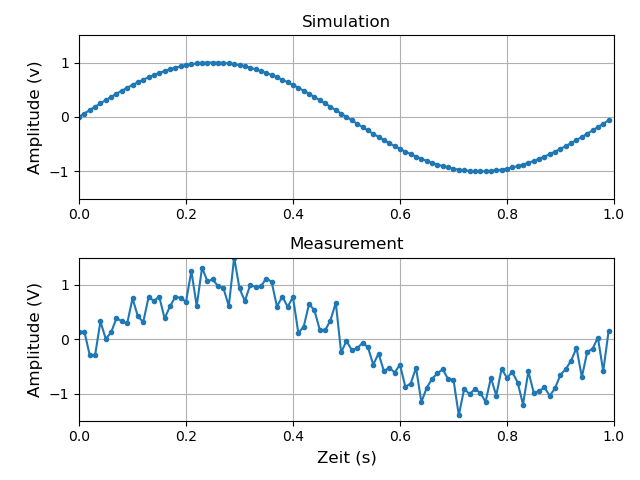
\includegraphics[width=8cm,align=t]{pics/Matplotlib/Subplots.png}
	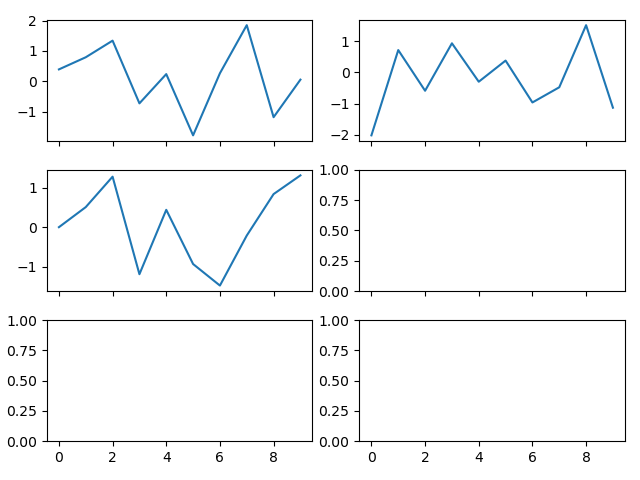
\includegraphics[width=8cm,align=t]{pics/Matplotlib/MultSubplots.png}
\end{minipage}
%%%%%%%%%%%%%%%%%%%%%%%%%%%%%%%%%%%%%%%%%%%%%%%%%%
\newpage
%%%%%%%%%%%%%%%%%%%%%%%%%%%%%%%%%%%%%%%%%%%%%%%%%%
\textbf{logarithmische Darstellung}
\\
\begin{minipage}[h]{10cm}
	\lstinputlisting{code/Matplotlib/Log.py}
\end{minipage}
\begin{minipage}[h]{8cm}
	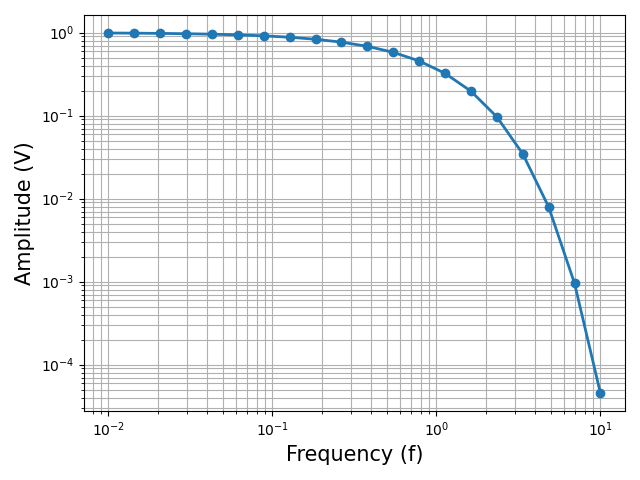
\includegraphics[width=7cm,align=t]{pics/Matplotlib/Loglog.png}
	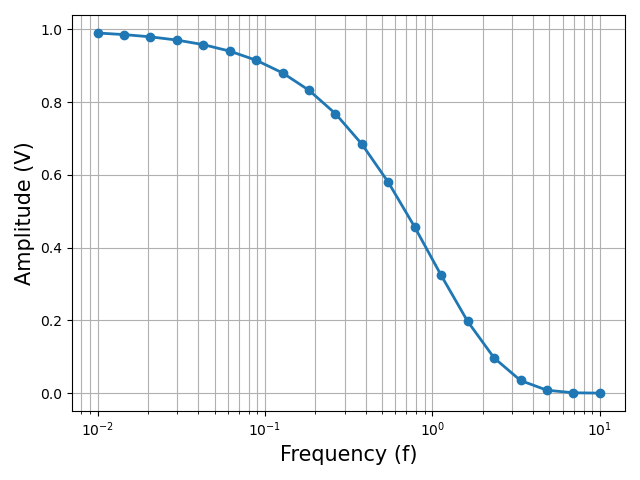
\includegraphics[width=7cm,align=t]{pics/Matplotlib/Semilogx.png}
\end{minipage}
%%%%%%%%%%%%%%%%%%%%%%%%%%%%%%%%%%%%%%%%%%%%%%%%%%
\\[0.1cm]
%%%%%%%%%%%%%%%%%%%%%%%%%%%%%%%%%%%%%%%%%%%%%%%%%%
\textbf{step}
\\
\begin{minipage}[h]{10cm}
	\lstinputlisting{code/Matplotlib/Step.py}
\end{minipage}
\begin{minipage}[h]{8cm}
	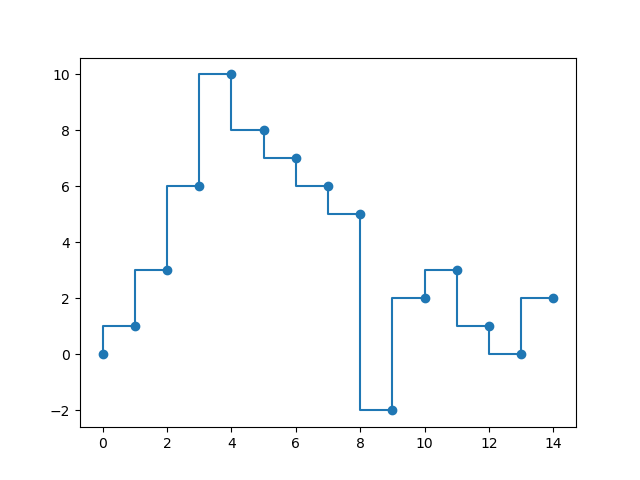
\includegraphics[width=7cm,align=t]{pics/Matplotlib/Step.png}
\end{minipage}
%%%%%%%%%%%%%%%%%%%%%%%%%%%%%%%%%%%%%%%%%%%%%%%%%%
\newpage
%%%%%%%%%%%%%%%%%%%%%%%%%%%%%%%%%%%%%%%%%%%%%%%%%%
\textbf{contour/contourf}
\\
\begin{minipage}[h]{10cm}
	\lstinputlisting{code/Matplotlib/Contour.py}
\end{minipage}
\begin{minipage}[h]{8cm}
	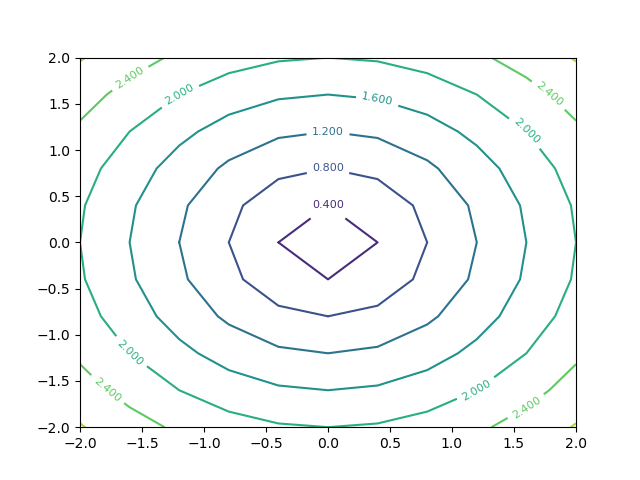
\includegraphics[width=7cm,align=t]{pics/Matplotlib/Contour.png}
	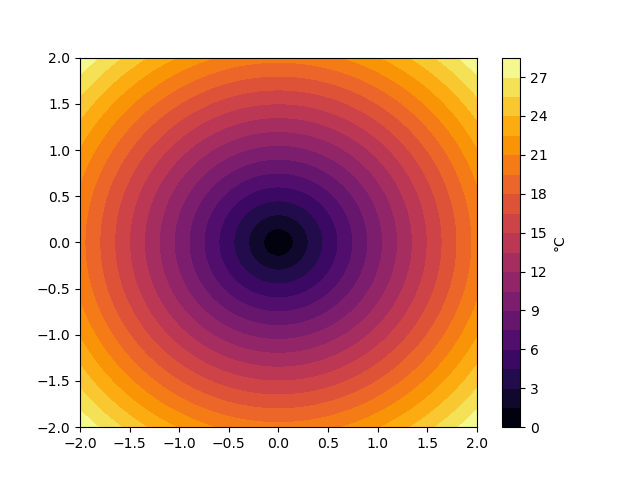
\includegraphics[width=7cm,align=t]{pics/Matplotlib/Contourf.png}
\end{minipage}
%%%%%%%%%%%%%%%%%%%%%%%%%%%%%%%%%%%%%%%%%%%%%%%%%%
\\[0.5cm]
%%%%%%%%%%%%%%%%%%%%%%%%%%%%%%%%%%%%%%%%%%%%%%%%%%
\textbf{hist}
\\[0.1cm]
\begin{minipage}[h]{10cm}
	\lstinputlisting{code/Matplotlib/Hist.py}
\end{minipage}
\begin{minipage}[h]{8cm}
	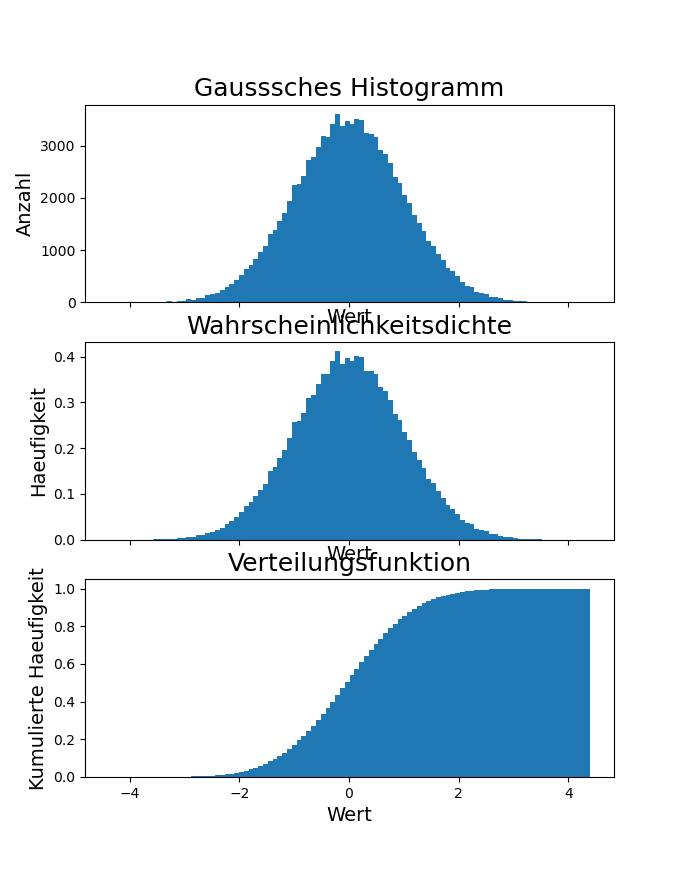
\includegraphics[width=8cm,align=t]{pics/Matplotlib/Hist.png}
\end{minipage}
%%%%%%%%%%%%%%%%%%%%%%%%%%%%%%%%%%%%%%%%%%%%%%%%%%
\newpage
%%%%%%%%%%%%%%%%%%%%%%%%%%%%%%%%%%%%%%%%%%%%%%%%%%
\textbf{scatter}
\\[0.1cm]
\begin{minipage}[h]{10cm}
	\lstinputlisting{code/Matplotlib/Scatter.py}
\end{minipage}
\begin{minipage}[h]{8cm}
	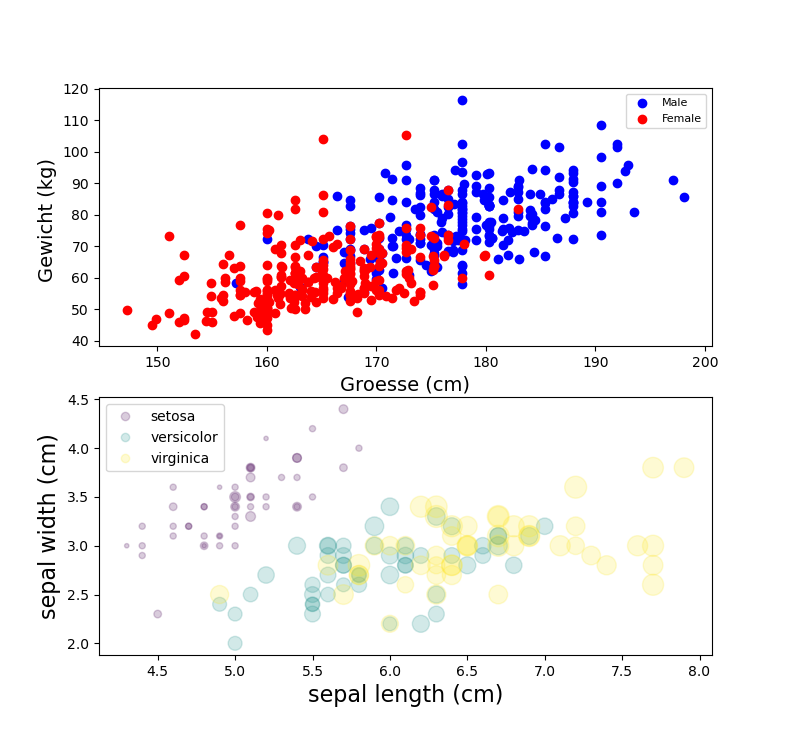
\includegraphics[width=10cm,align=t]{pics/Matplotlib/Scatter.png}
\end{minipage}
%%%%%%%%%%%%%%%%%%%%%%%%%%%%%%%%%%%%%%%%%%%%%%%%%%
\end{document}